\chapter{Hamiltonian Path/Cycle}
Ajur was walking with Jura thinking what he could do to inspire a problem to be named after himself. Rishnak found Ajur to be an interesting youngster to discuss puzzles based on Graph Theory. After the discussion of the Eulerian Walk, Rishnak decided to introduce a closely related graph-theoretic construction: Hamiltonian Paths and Hamiltonian Cycles. Rishank approached Ajur and Jura and began defining the notion of a Hamiltonian path and Hamiltonain walk.
In a Hamiltonian path each of the vertices are visited exactly once. 
The length of a path is the number of edges in that path. A Hamiltonian path in a graph with $n$ vertices will have a path length of $n-1$. A Hamiltonian cycle is a cycle that visits each vertex once and only once. The length of a Hamiltonian Cycle in a graph with $n$ vertices is $n$. Rishnak asked Ajur whether there is a Hamiltonian cycle in the graph of Figure \ref{5g1},
\begin{figure}
\begin{center}
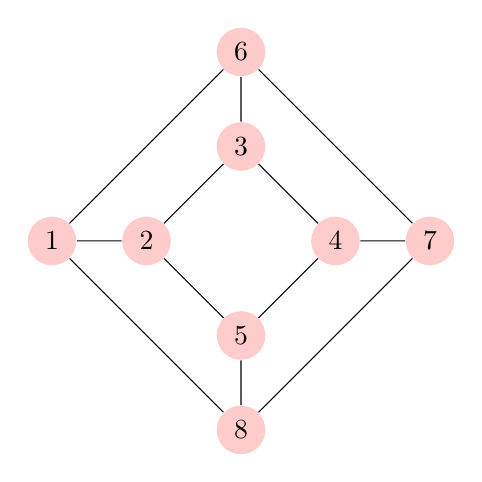
\begin{tikzpicture}
  [scale=.6,auto=left,every node/.style={circle,fill=red!20}]
  \node (n1) at (1,7) {1};
  \node (n2) at (3,7)  {2};
  \node (n4) at (7,7) {4};
  \node (n7) at (9,7)  {7};
  \node (n6) at (5,11)  {6};
   \node (n3) at (5,9) {3};
   \node (n5) at (5,5) {5};
   \node (n8)  at (5,3) {8};
  \foreach \from/\to in {n1/n2,n2/n3,n3/n4,n4/n5,n5/n2,n1/n6,
  n6/n7, n7/n8, n8/n1, n3/n6, n4/n7, n5/n8}
    \draw (\from) -- (\to);

\end{tikzpicture}
\caption{ Cube Graph }\label{5g1}
\end{center}
\end{figure}

Ajur thought about for a few seconds and he drew the Hamiltonian cycle of Figure \ref{5g1} in Figure \ref {5g2}. Krishnak told Ajur that his solution is not unique and there are more solutions!\footnote{Try to find a Hamiltonian Cycle distinct from the one described by Ajur!}

\begin{figure}
\begin{center}
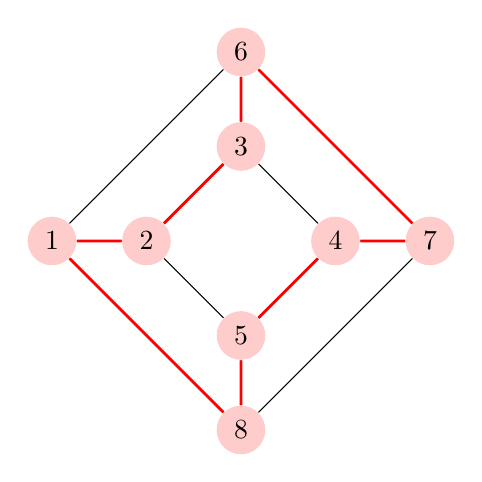
\begin{tikzpicture}
  [scale=.6,auto=left,every node/.style={circle,fill=red!20}]
  \node (n1) at (1,7) {1};
  \node (n2) at (3,7)  {2};
  \node (n4) at (7,7) {4};
  \node (n7) at (9,7)  {7};
  \node (n6) at (5,11)  {6};
   \node (n3) at (5,9) {3};
   \node (n5) at (5,5) {5};
   \node (n8)  at (5,3) {8};
  \foreach \from/\to in {n1/n2,n2/n3,n3/n4,n4/n5,n5/n2,n1/n6,
  n6/n7, n7/n8, n8/n1, n3/n6, n4/n7, n5/n8}
    \draw (\from) -- (\to);
\path[line width=0.35mm,red] (n1) edge (n2)
(n2) edge (n3)
(n3) edge (n6)
(n6) edge (n7)
(n7) edge (n4)
(n4) edge (n5)
(n5) edge (n8)
(n8) edge (n1);
\end{tikzpicture}
\caption{ Cube Graph with Hamiltonian  Cycle marked in thick edges}\label{5g2}
\end{center}
\end{figure}

Rishnak then told Ajur what led Hamilton to the statement of the Hamiltonian cycle problem. The mathematician Hamilton wanted a cycle to visit 
all the vertices of a dodecahedron (one of the five platonic solids) which has 20 vertices and 30 edges. 
Rishnak asked Ajur whether there is a Hamiltonian Cycle in the graph of Figure \ref{5g3}. Rishnak added that this is a well-known graph, called the Petersen Graph.

\begin{figure}
\begin{center}
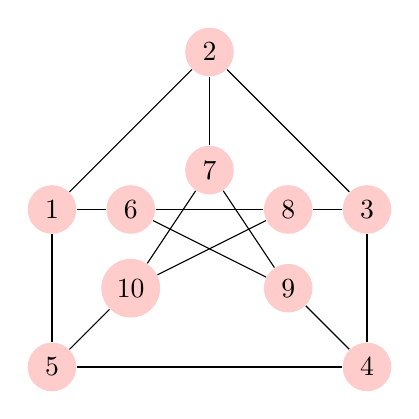
\begin{tikzpicture}
  [scale=.5,auto=left,every node/.style={circle,fill=red!20}]
  \node (n1) at (1,7) {1};
  \node (n2) at (5,11)  {2};
  \node (n3) at (9,7)  {3};
  \node (n4) at (9,3) {4};
  \node (n5) at (1,3) {5};
  \node (n6) at (3,7)  {6};
  \node (n7) at (5,8) {7};
  \node (n8)  at (7,7) {8};
  \node (n9) at (7,5) {9};
  \node (n10) at  (3,5) {10};
 
  \foreach \from/\to in {n1/n2,n2/n3,n3/n4,n4/n5,n5/n1,n1/n6,
  n2/n7, n3/n8, n4/n9, n5/n10, n6/n8, n8/n10, n10/n7,n7/n9,n9/n6}
    \draw (\from) -- (\to);

\end{tikzpicture}
\caption{ Petersen Graph with 10 vertices and 15 edges }\label{5g3}
\end{center}
\end{figure}
Ajur thought for a while and he was not able to construct a Hamiltonian cycle. He however, was able to find a 
Hamiltonian path. So he drew the following Figure \ref{5g4}. Rishnak mentioned to Ajur that this Hamiltonian path is not unique and there are other Hamiltonian paths.\footnote{Find a Hamiltonian path distinct from the one shown here.}


\begin{figure}
\begin{center}
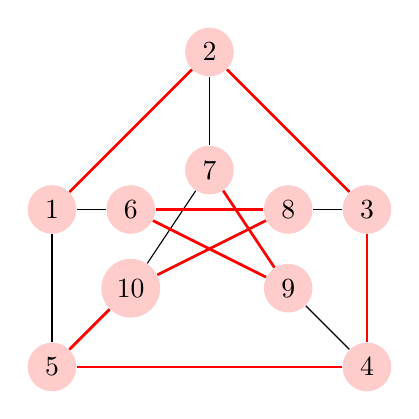
\begin{tikzpicture}
  [scale=.5,auto=left,every node/.style={circle,fill=red!20}]
  \node (n1) at (1,7) {1};
  \node (n2) at (5,11)  {2};
  \node (n3) at (9,7)  {3};
  \node (n4) at (9,3) {4};
  \node (n5) at (1,3) {5};
  \node (n6) at (3,7)  {6};
  \node (n7) at (5,8) {7};
  \node (n8)  at (7,7) {8};
  \node (n9) at (7,5) {9};
  \node (n10) at  (3,5) {10};
 
  \foreach \from/\to in {n1/n2,n2/n3,n3/n4,n4/n5,n5/n1,n1/n6,
  n2/n7, n3/n8, n4/n9, n5/n10, n6/n8, n8/n10, n10/n7,n7/n9,n9/n6}
    \draw (\from) -- (\to);
\path[line width=0.35mm,red]
(n1) edge (n2)
(n2) edge (n3)
(n3) edge (n4)
(n4) edge (n5)
(n5) edge (n10)
(n10) edge (n8)
(n8) edge (n6)
(n6) edge (n9)
(n9) edge (n7);

\end{tikzpicture}
\caption{ Petersen Graph with a Hamiltonian Path}\label{5g4}
\end{center}
\end{figure}
Rishnak assured Ajur that Petersen Graph indeed does not have a Hamiltonian cycle. Whether a graph has an Eulerian Cycle or not can easily be tested (the degree of every vertex has to be even); however, there is no easy way for test whether a given graph has a Hamiltonian cycle. 

Rishnak continued that there is a special class of graphs called bipartite graphs where every cycle is of even length. The vertex set can be partitioned into two sets $A$ and $B$, such that every edge in such a graph has one end vertex in $A$ and the other end vertex in $B$. Rishnak showed an example in Figure \ref{5g5}. Ajur immediately said that all the cycles are of even lengths (4 and 6).\footnote{Every edge in the cycle must go from one partition to the other partition (as they are the only possible edges). Hence the length of a cycle must be even.} Rishnak asked Ajur what the two vertex partitions are (all the edges go from one partition to the other). After a little thought Ajur said one partition contains 1, 3, 5 and the other partition contains the vertices 2, 4 and 6. Ajur drew a graph (see Figure \ref{5g55}) to illustrate  what he meant. Ajur also mentioned that this graph has a Hamiltonian cycle.\footnote{Ajur exclaimed that every tree is a bipartite graph too, as a tree contains no cycles (or cycles of length 0 - we know that 0 is an even number!). Rishnak reminded Ajur that since tree does not have cycles and hence no Hamiltonian cycles.} 
Ajur wanted to show that he had understood the concept of a bipartite graph. So he drew a graph that does not have a Hamiltonian cycle - see Figure \ref{5g6}. Ajur explained why this graph does not have a Hamiltonian cycle. If there were a Hamiltonian cycle, the vertices in the cycle have to alternate between the two vertex partitions. But one vertex partition has two vertices and the other vertex partition has three vertices. Rishnak smiled and appreciated Ajur's logical thinking.

\begin{figure}
\begin{center}
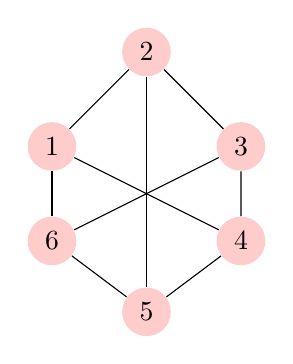
\begin{tikzpicture}
  [scale=.3,auto=left,every node/.style={circle,fill=red!20}]
  \node (n1) at (1,7) {1};
  \node (n2) at (5,11)  {2};
  \node (n3) at (9,7)  {3};
  \node (n4) at (9,3) {4};
  \node (n5) at (5,0)  {5};
  \node (n6) at (1,3) {6};
  
   \foreach \from/\to in {n1/n2,n2/n3,n3/n4,n4/n5,n5/n6,n1/n6,
  n2/n5, n6/n3,n1/n4}
    \draw (\from) -- (\to);
    \end{tikzpicture}
\caption{ A Bipartite Graph with 6 vertices and 9 edges}\label{5g5}
\end{center}
\end{figure}
\begin{figure}
\begin{center}
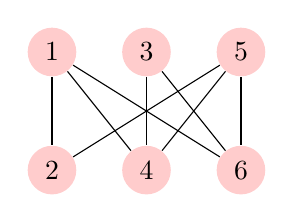
\begin{tikzpicture}
  [scale=.3,auto=left,every node/.style={circle,fill=red!20}]
  \node (n1) at (1,7) {1};
  \node (n3) at (5,7)  {3};
  \node (n5) at (9,7) {5};
  \node (n2) at (1,2)  {2};
  \node (n4) at (5,2) {4};
  \node (n6) at (9,2)  {6};
 
  
   \foreach \from/\to in {n1/n2,n1/n4,n1/n6,n3/n4,n3/n6,n5/n2,n5/n4,n5/n6}
    \draw (\from) -- (\to);
    \end{tikzpicture}
\caption{ Graph in \ref{5g5} drawn with vertex partition}\label{5g55}
\end{center}
\end{figure}
\begin{figure}
\begin{center}
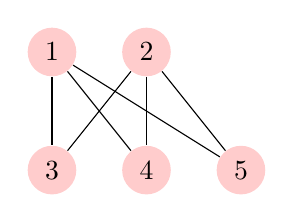
\begin{tikzpicture}
  [scale=.3,auto=left,every node/.style={circle,fill=red!20}]
  \node (n1) at (1,7) {1};
  \node (n2) at (5,7)  {2};
  \node (n3) at (1,2)  {3};
  \node (n4) at (5,2) {4};
  \node (n5) at (9,2)  {5};
 
  
   \foreach \from/\to in {n1/n3,n1/n4,n1/n5,n2/n3,n2/n4,n2/n5}
    \draw (\from) -- (\to);
    \end{tikzpicture}
\caption{ A Bipartite Graph with 5 vertices and 6 edges}\label{5g6}
\end{center}
\end{figure}

Rishnak decided to tell Ajur a simplified version of a puzzle\footnote{attributed to Bruce Robinson, a professor of civil and environmental engineering at the University of Tennessee.} he had heard in the radio program Car Talk (broadcast on public radio). There are 9 jealous people who live in the squares of a three-by-three grid (see Figure \ref{5g7}. The squares are numbered, starting on the upper left-hand corner, 1 through 9 (first going across). Each person is jealous of his adjacent neighbor; we emphasize not his diagonal neighbor, but only the people above, below, or to the right or to the left of him. Each aspires to move into the apartment of an adjacent neighbor.
The question is very simple: What is the fewest number of total moves that can accomplish this?
\begin{figure}
\begin{center}
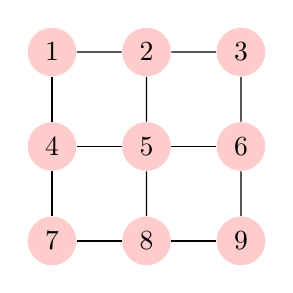
\begin{tikzpicture}
  [scale=.3,auto=left,every node/.style={circle,fill=red!20}]
  \node (n1) at (1,11) {1};
  \node (n2) at (5,11)  {2};
  \node (n3) at (9,11) {3};
  \node (n4) at (1,7)  {4};
  \node (n5) at (5,7) {5};
  \node (n6) at (9,7)  {6};
  \node (n7) at (1,3)  {7};
  \node (n8) at (5,3) {8};
  \node (n9) at (9,3)  {9};
  
  
   \foreach \from/\to in {n1/n2,n1/n4,n2/n3,n2/n5,n3/n6,n4/n5,n4/n7,n5/n6,n5/n8,n6/n9,n7/n8,
   n8/n9}
    \draw (\from) -- (\to);
    \end{tikzpicture}
\caption{ A three by three grid with nine apartments. Apartments are modeled as vertices and an edge denotes adjacency relation between apartments (up, down, two sides - not all apartments have all of the adjacent apartments} \label{5g7}
\end{center}
\end{figure}

Ajur immediately figured  this is a bipratite graph and the partitions are not of equal size. Hence immediately he responded that this is not possible. Rishnak asked Ajur to write down the argument to make sure it is correct. Ajur promised that he would do it by next day. This graph has a Hamiltonian path but not a Hamiltonian cycle. Ajur said that instead of three by three grid of apartments, if we had a four by three grid (or three by four grid) of apartments, it is easy for all of them to transfer to the adjacent apartments. Such a graph has a Hamiltonian cycle. \textbf{why?}

Rishnak continued with other related puzzles. Euler proposed the \emph{Knight's tour} problem on a chessboard. A chessboard is an eight by eight square grid. Place a knight in any square. From that square, the knight has to move\footnote{knight may only move either two squares vertically up/down and one square horizontally left or right or one square vertically up or down and two squares horizontally left or right. More coloquially, a knight moves in a 2x1 L shape} visiting all of the squares squares exactly. One may think of this as finding a Hamiltonian path in a 64-vertex graph with two vertices adjacent if there is a knight move from one vertex to the other. There is no easy method of finding a knight's tour other than exhaustive search.\footnote{The usual method of exhaustive search is through backtracking - a systematic method of exploring all possibilities.} Here is a solution in Table \ref{5t1} for a five by five chess board with the knight's tour starting from bottom left.
\begin{table}
\centering
\begin{tabular}{|c |c |c| c| c|} 
 \hline
3&10&21&16& 5\\
\hline
20&15& 4&11&22\\
\hline
 9& 2&23& 6&17\\
 \hline
14&19& 8&25&12\\
\hline
 1&24&13&18& 7\\
 \hline
\end{tabular}
\caption{Knight's Tour on five by five chess board starts at the bottom left}
\label{5t1}
\end{table}
Rishnak asked Ajur to find the message is encoded here in Table \ref{5t2}.
\begin{table}
\centering
\begin{tabular}{c c c c cc}
i& t& t& t& b& l\\
r& h &d &e& u& s\\
h& a& y& e& d& o\\
a& o& e& p& r& n\\
s& n& f& o& l& l\\
f& v& d &i& e& u\\
\end{tabular}
\caption{What is the Message is encoded here}
\label{5t2}
\end{table}
Rishnak added that there are poems from different cultures (including India and China) based on Knight's tour. Ajur was intrigued and resolved to read and understand the poems. Rishnak added that one needs to verify that a knight's tour is impossible for a three by three chessboard or a four by four chessboard and warned that checking whether a knight's tour is impossible may take a long time.

There are many methods to check whether a given graph has a Hamiltonian cycle. Unfortunately these conditions are \textbf{not} exhaustive. Rishnak taught Ajur a simple test to know whether a graph has a Hamiltonian cycle.

Rishnak stated a well-known theorem that if the degree of every vertex in a graph with $n$ vertices is at least$\frac{n}{2}$, then the graph has a Hamiltonian cycle. The main proof argument consists of three parts.
\begin{enumerate}
    \item First one shows the graph is connected.
    \item The length of the longest path in any graph with $n$ vertices is $\le n-1$.
    \item If $\mathcal{P}$ is a longest path, then one can find a Hamiltonian cycle.
\end{enumerate}


First the graph has to be connected - Otherwise there will be at least two connected components, one of which will have size at most $\frac{n}{2}$, violating the degree condition. In this connected graph, find the longest path. Let it be $v_1,v_2,\cdots, v_k$. Since this is the longest path, all the neighbors of the starting vertex $v_1$ and the ending vertex $v_k$ have  to be in this path. Otherwise we could have extended that path and hence the path we started with is not the longest path. Hence at least $\frac{n}{2}$ vertices in the path $v_2,v_3,\cdots,v_k$ are adjacent to $v_0$. Let those adjacent vertices of $v_1$ form set $S_1$= $\{v_i,v_j,\cdots v_m\}$. The size of this set is at least $\frac{n}{2}$. For each of these vertices, consider their preceding vertices in the path. Let that set be $S_2$. The size of that set is also at least $\frac{n}{2}$. The vertices adjacent to $v_k$ have to be a set of size at least $\frac{n}{2}$ and they are among $v_1,v_2,\cdots v_{k-1}$. If none of the vertices adjacent to $v_k$ are in set $S_2$, then the vertices adjacent to $v_k$ would have size < $\frac{n}{2}$ because $k-1-\frac{n}{2} <\frac{n}{2}$. Hence we would have a situation as shown in Figure \ref{5g100}
\begin{figure}
\begin{center}
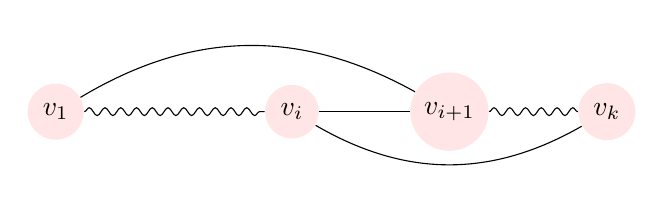
\begin{tikzpicture}
  [scale=.5,auto=left,every node/.style={circle,fill=red!10}]
  \node (n1) at (-1,11) {$v_1$};
  \node (n2) at (5,11)  {$v_i$};
  \node (n3) at (9,11) {$v_{i+1}$};
  \node (n4) at (13,11) {$v_k$};
  
  

    \draw (n2) -- (n3);
   \path (n1) edge[bend left=30] (n3);
    \path (n2) edge[bend right=30] (n4);
    \tikzset{decoration={snake,amplitude=.5mm,segment length=2mm,
                       post length=0mm,pre length=0mm}}
  \draw[decorate] (n1) -- (n2);
  \draw[decorate] (n3) -- (n4);
    \end{tikzpicture}
\caption{ Pictorial Description of the argument; solid lines represent edges, squiggly lines represent paths} \label{5g100}
\end{center}
\end{figure}
 
This creates a cycle $v_k,v_i,\cdots,v_1,v_{i+1}\cdots, v_k$ as shown in \ref{5g100}. The claim is that this is a Hamiltonian Cycle. If not there is at least one vertex in this cycle that will be adjacent to some other vertex. This will result in a path longer than the path we originally started - a contradiction.
Ajur was able to follow along and loved the subtle and the clever arguments used in the proof. 


But Jura who was patiently waiting was beginning to get restless so Ajur called it a day.
